\chapter{Methods}
\label{chap:phage_methods}

This chapter introduces the reaction-diffusion model used in this part of the thesis, explaining the necessary coupling terms to describe bacteria-phage interactions and the non-dimensional version of it. Then we will introduce the chemostat version of it, used to model a similar system in a well-mixed environment. Furthermore, we will introduce the respective observables which were defined to quantify results obtained from the ensuing dynamics.
\section{Model}
The interactions within our model are graphically depicted in Figure \ref{fig:model_sketch} while excluding diffusion and nutrients in the sketch for simplicity.
\begin{figure}
\centering
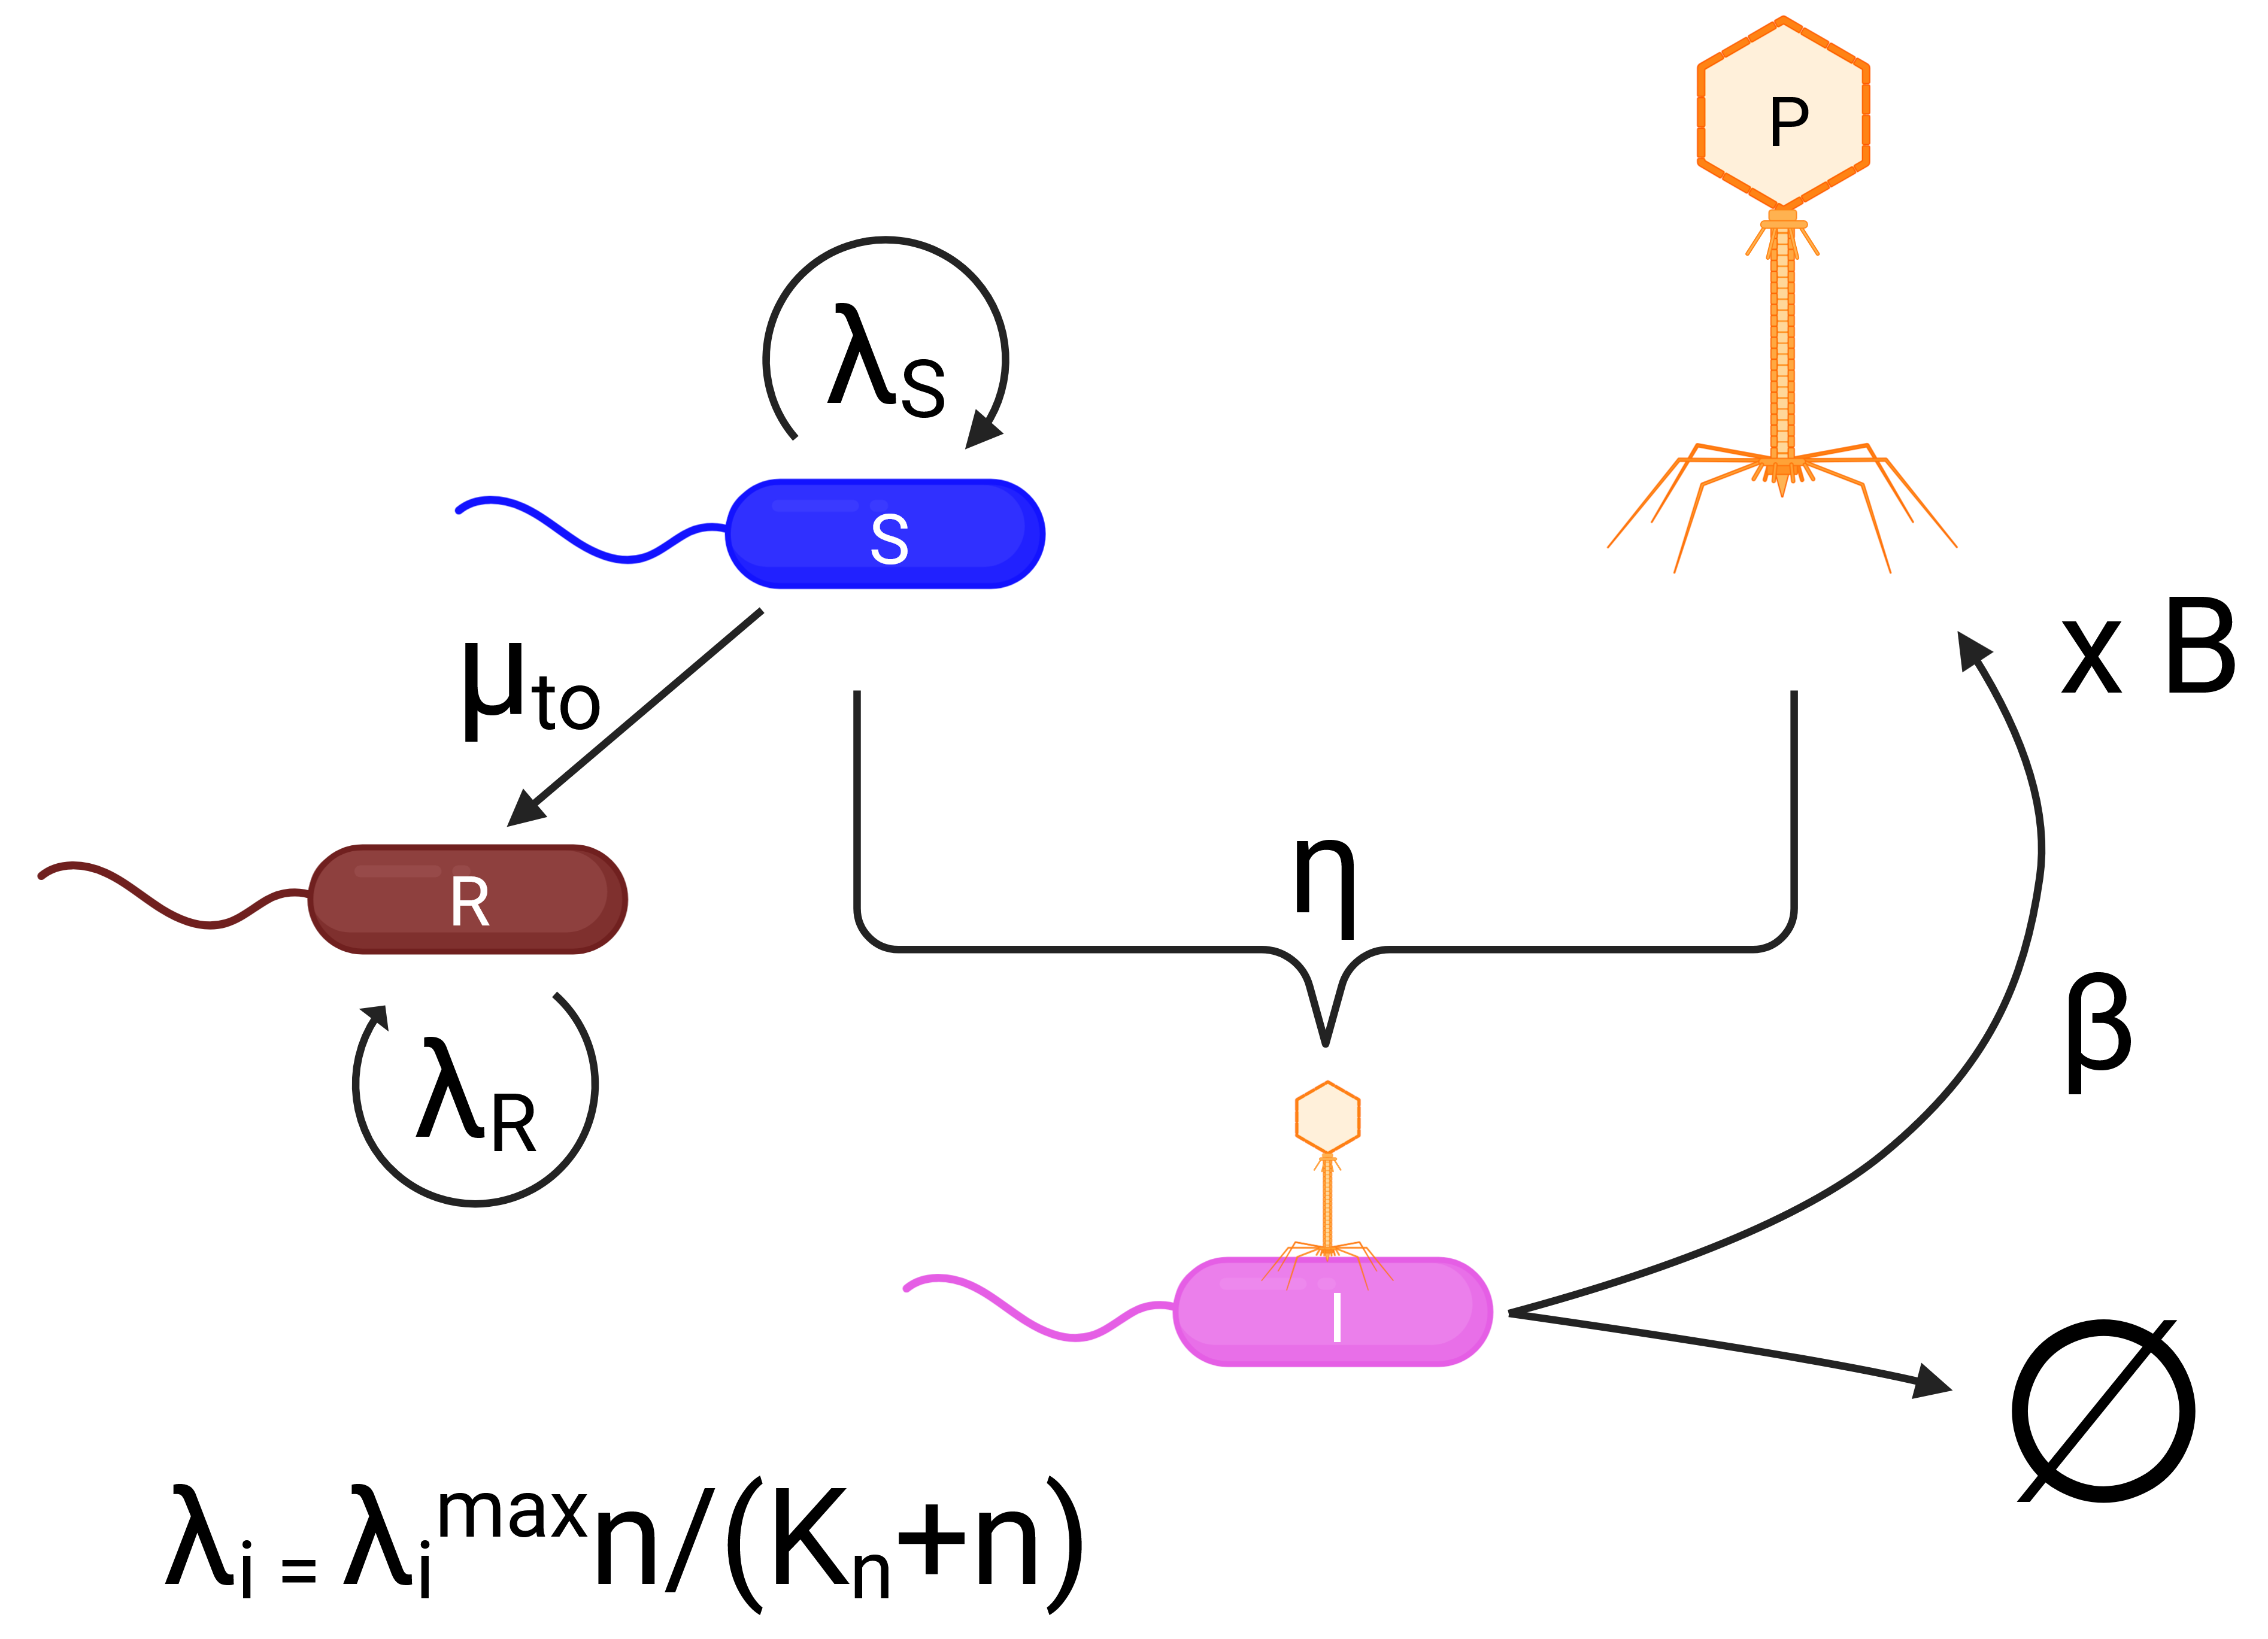
\includegraphics[width=\linewidth]{graphics/2025_09_30_phages_fig1.png}
\caption{\textbf{Sketch of the reaction-diffusion model} Sensitive bacteria, depicted in blue, grow with a growth rate $\lambda_s$ and are infected by phages, depicted in orange, with an infection rate $\eta$. This infection process forms infected bacteria, depicted in pink, which burst with a burst rate $\beta$ and upon lysis release $B$ new phages. In addition resistant bacteria, depicted in brown, are present in the system, grow with a growth rate $\lambda_r$ and sensitive bacteria can mutate to become resistant with mutation rate $\mu_{to}$. Both growth rates are changing depending on nutrient availability.}
\label{fig:model_sketch}
\end{figure}
Our model is most similar to the model used to describe the hitchhiking effect of phages in bacteria~\cite{Ping2020-vd} and is given by the following set of~\gls{pde}s:
\begin{align}
    \frac{\text{d}S}{\text{d}t} = D_b &\frac{\partial^2S}{\partial x^2} + \left( 1 - \mu_{to} \right) \lambda_s S \frac{n}{K_n+n}  - \eta SP \\
    \frac{\text{d}I}{\text{d}t} = D_b &\frac{\partial^2I}{\partial x^2} + \eta SP - \beta I\\
    \frac{\text{d}R}{\text{d}t} = D_r &\frac{\partial^2R}{\partial x^2} + \left[\lambda_r R + \mu_{to} \lambda_s S \right] \frac{n}{K_n+n}\\
    \frac{\text{d}P}{\text{d}t} = D_p &\frac{\partial^2P}{\partial x^2} + \beta BI - \eta P(S+I) \\
    \frac{\text{d}n}{\text{d}t} = D_n &\frac{\partial^2n}{\partial x^2} - \frac{1}{Y} \left( \lambda_s S + \lambda_r R \right) \frac{n}{K_n+n}
\end{align}
where $D_b$, $D_p$ and $D_n$ are the respective diffusion rates, $\mu_{to}$ and $\mu_{back}$ are the towards and backwards mutation rates, $\lambda_S$ and $\lambda_R$ are the respective growth rates, $K_n$ is the half-velocity constant, $\eta$ is the infection rate, $\beta$ is the lysis rate, $B$ is the burst size and $Y$ is the nutrient yield. To improve readability, we omit dependencies on space and time for all variables. The model can easily be generalized to multiple dimensions but we focus here on the most simple one-dimensional case.

These equations can be non-dimensionalized using the following transformations for space, time and quantities:\\
% \begin{align*}
%     x &\rightarrow \tilde{x} = \sqrt{\frac{D_b}{\lambda_s}} x \\
%     t &\rightarrow \tilde{t} = \frac{1}{\lambda_s} \\
%     S &\rightarrow \tilde{S} = K_n Y S \\
%     I &\rightarrow \tilde{I} = K_n Y I \\ 
%     R &\rightarrow \tilde{R} = K_n Y R \\
%     P &\rightarrow \tilde{P} = \frac{\lambda_s}{\eta} P \\
%     n &\rightarrow \tilde{n} = K_n n
% \end{align*}
$x \rightarrow \tilde{x} = \sqrt{\frac{D_b}{\lambda_s}} x$, $t \rightarrow \tilde{t} = \frac{1}{\lambda_s}$, \\
$S \rightarrow \tilde{S} = K_n Y S$, $I \rightarrow \tilde{I} = K_n Y I$, $R \rightarrow \tilde{R} = K_n Y R$, $P \rightarrow \tilde{P} = \frac{\lambda_s}{\eta} P$, $n \rightarrow \tilde{n} = K_n n$\\
Then we can redefine parameters as:\\
% \begin{align*}
%     \tilde{D_p} &= \frac{D_p}{D_b} \\
%     \tilde{D_r} &= \frac{D_r}{D_b} \\
%     \tilde{D_n} &= \frac{D_n}{D_b} \\
%     \tilde{\beta} &= \frac{\beta}{\lambda_s} \\
%     \tilde{\eta} &= \frac{\eta K_n Y}{\lambda_s} \\
%     \tilde{\lambda_r} &= \frac{\lambda_r}{\lambda_s} \\
%     \tilde{B} &= B
% \end{align*}
$\tilde{D_p} = \frac{D_p}{D_b}$, $\tilde{D_r} = \frac{D_r}{D_b}$, $\tilde{D_n} = \frac{D_n}{D_b}$, $\tilde{\beta} = \frac{\beta}{\lambda_s}$, $\tilde{\eta} = \frac{\eta K_n Y}{\lambda_s}$, $\tilde{\lambda_r} = \frac{\lambda_r}{\lambda_s}$, $\tilde{B} = B$\\
and we can write the non-dimensionalized set of coupled~\gls{pde}s, when dropping the tilde, as:
\begin{align}
    \frac{\text{d}S}{\text{d}t} &= \frac{\partial^2S}{\partial x^2} + \left( 1 - \mu_{to} \right) S \frac{n}{1+n}  - SP \\
    \frac{\text{d}I}{\text{d}t} &= \frac{\partial^2I}{\partial x^2} + SP - \beta I\\
    \frac{\text{d}R}{\text{d}t} &= D_r \frac{\partial^2R}{\partial x^2} + \left[\lambda_r R + \mu_{to} S \right] \frac{n}{1+n}\\
    \frac{\text{d}P}{\text{d}t} &= D_p \frac{\partial^2P}{\partial x^2} + \beta \eta BI - \eta P(S+I) \\
    \frac{\text{d}n}{\text{d}t} &= D_n \frac{\partial^2n}{\partial x^2} - \left( S + \lambda_r R \right) \frac{n}{1+n}
\end{align}
For the well-mixed scenario, we drop the diffusion terms, add chemostat balancing terms and after analogous non-dimensionalization, we obtain the following set of~\gls{ode}s:
\begin{align}
    \frac{\text{d}S}{\text{d}t} &= \left( 1 - \mu_{to} \right) S \frac{n}{1+n}  - SP - d S\\
    \frac{\text{d}I}{\text{d}t} &= SP - \beta I - d I\\
    \frac{\text{d}R}{\text{d}t} &= \left[\lambda_r R + \mu_{to} S \right] \frac{n}{1+n} - d R\\
    \frac{\text{d}P}{\text{d}t} &= \beta \eta BI - \eta P(S+I) -d P\\
    \frac{\text{d}n}{\text{d}t} &= - \left( S + \lambda_r R \right) \frac{n}{1+n} - d n
\end{align}
For our simulations, unless noted otherwise, we use the following parameter values (after non-dimensionalization):
$D_p = 1/18$, $D_r = 1$, $D_n = 50/3$, $\beta = 50/13$, $\lambda_r = 1$, $B = 70$, $\eta = 2/65$, $\mu_{to} = 0.01$
Numerical simulations of the equations were performed in python, using \text{scipy.solve\_ivp()} with a flexible time step ran until a time $t_{max}$ and a discretization of space with $N$ discretization points and stepping size $dx$.
Commonly, we use $t_{max} = 910$, $N = 600$ and $dx = \sqrt{65}/6$.

\section{Observables}
\begin{figure}
\centering
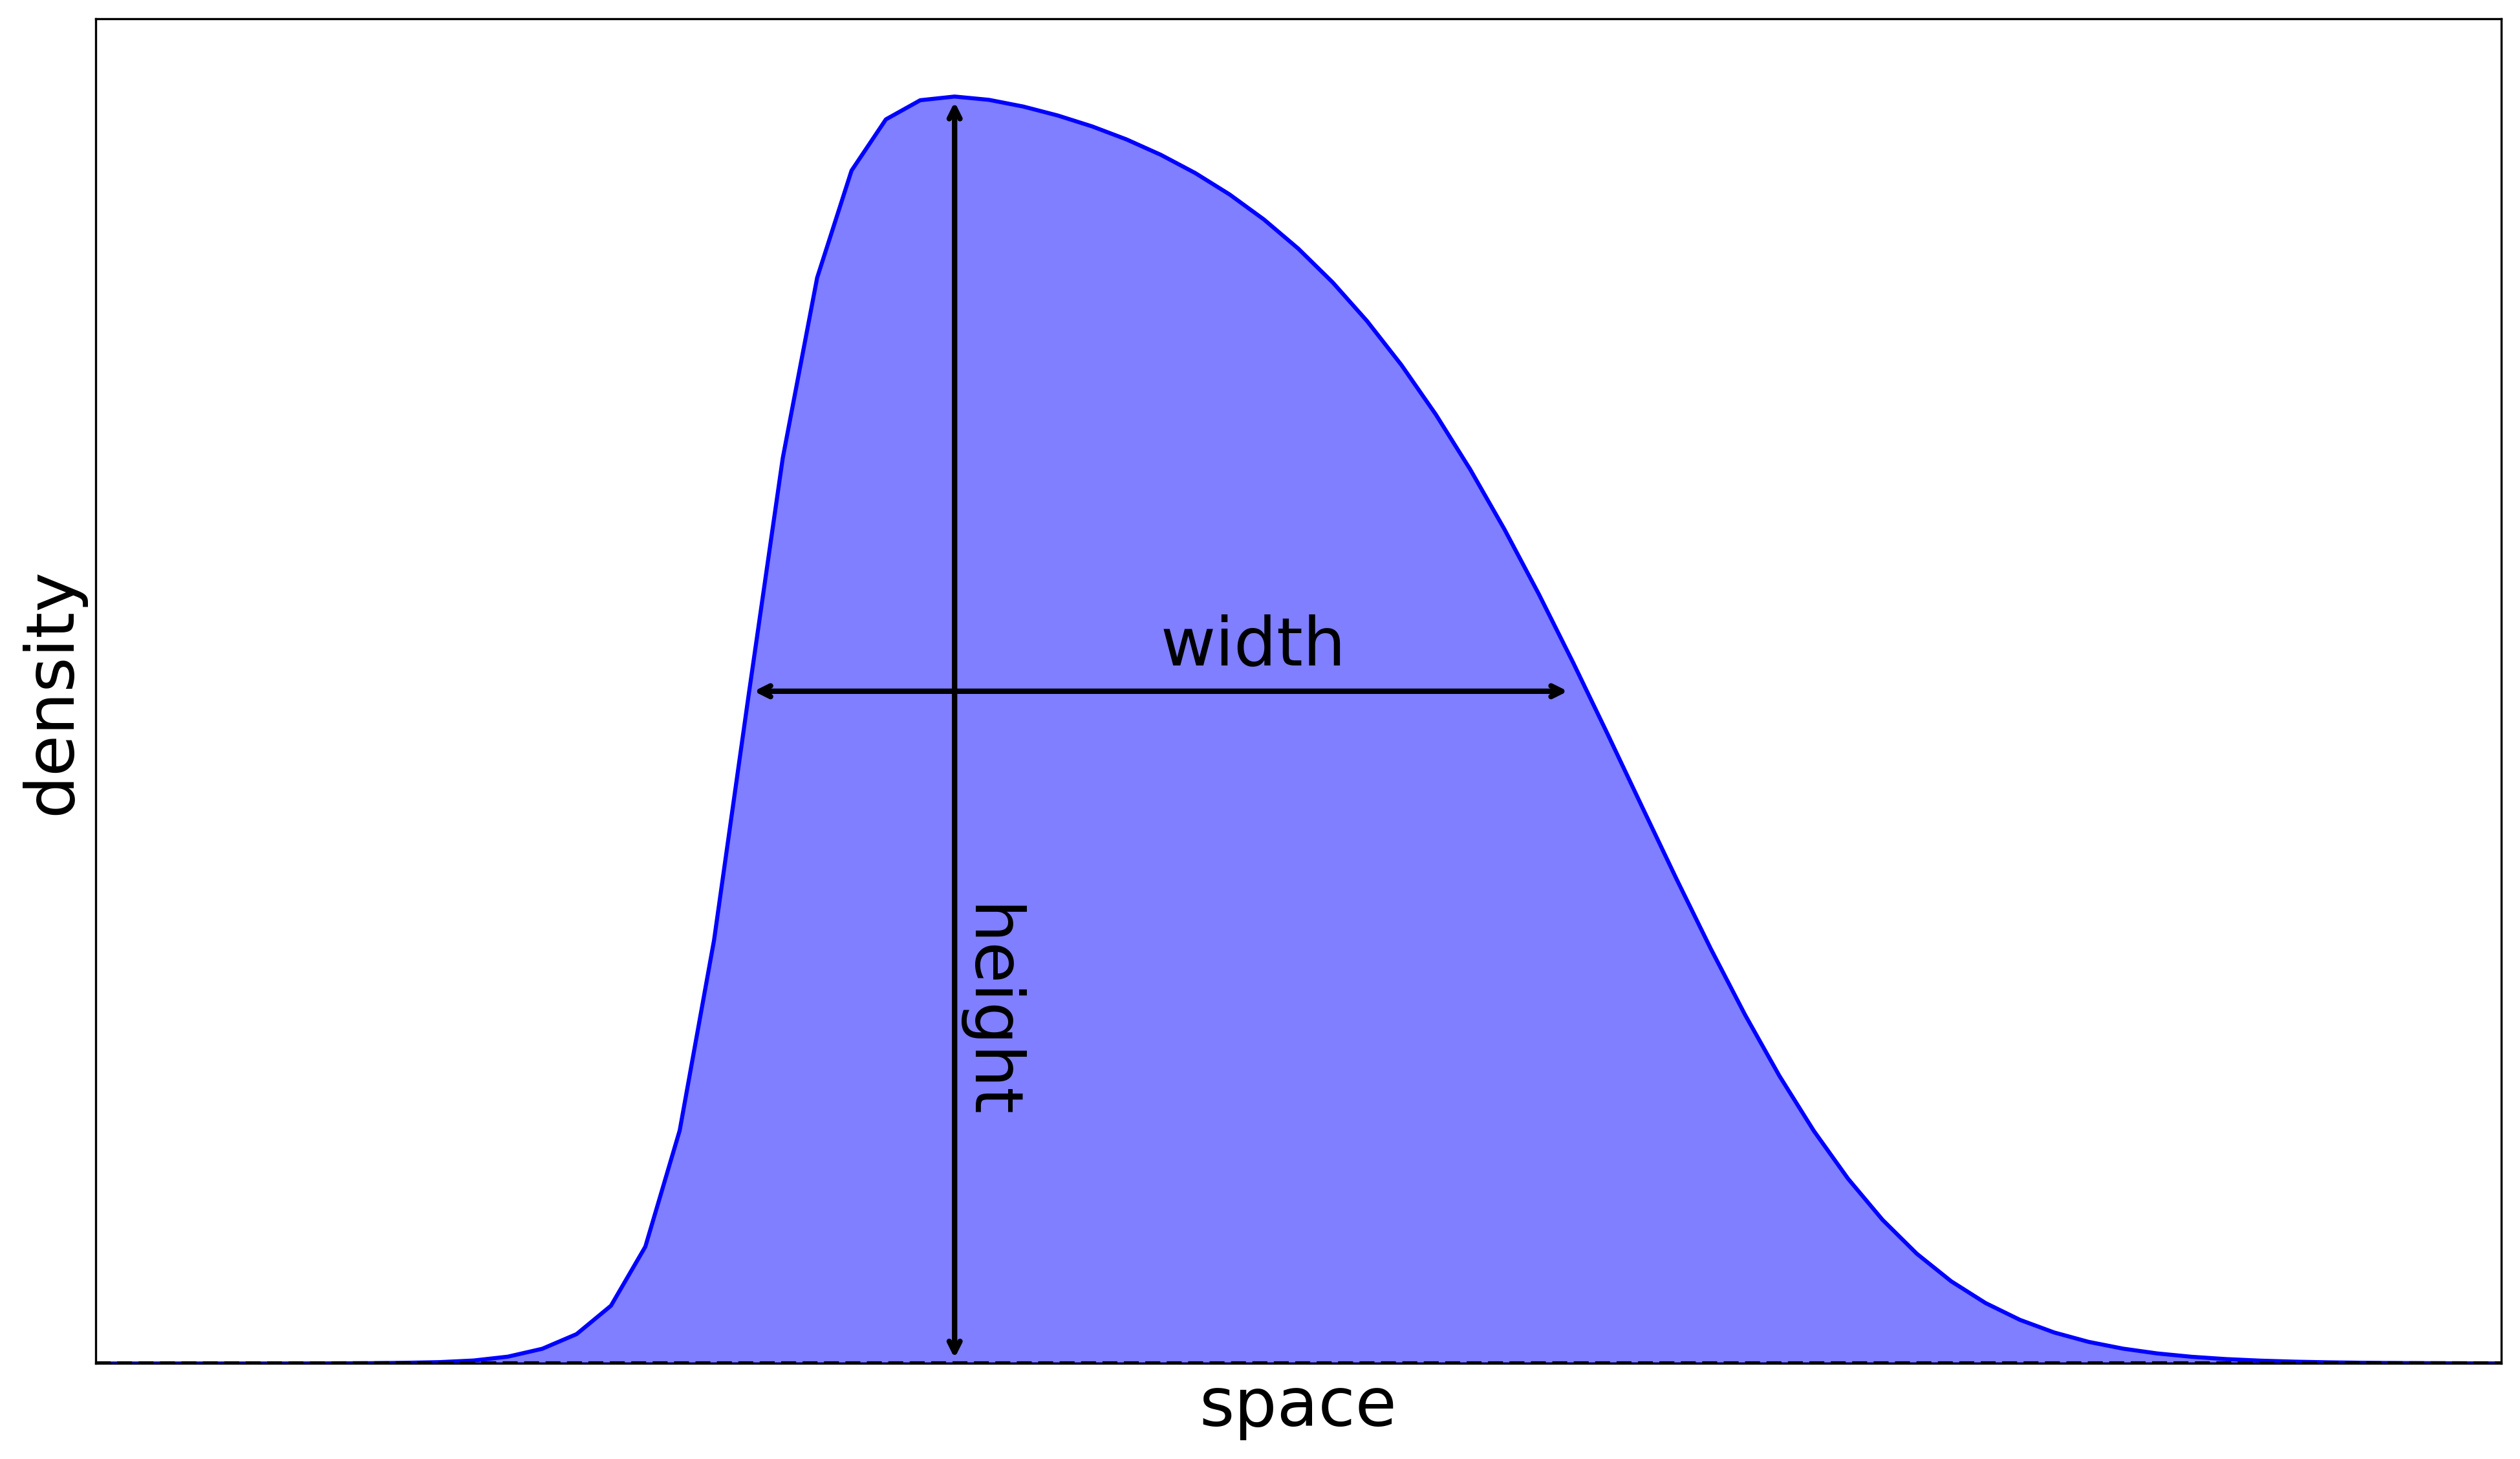
\includegraphics[width=\linewidth]{graphics/2025_09_30_phages_fig2.png}
\caption{\textbf{Example time snapshot for a traveling wave in the dynamics} The shaded area is the amount of bacteria or phages we measure and in addition the maximum of the wave is measured as the height and the width is measured.}
\label{fig:observable_sketch}
\end{figure}
We describe and quantify the dynamics being created by solving our model system using three observables for the forming traveling wave. We measure the amount of bacteria which is represented as the area under the curve and additionally we measure the height and the width at 1e-6 of the maximum of the curve as represented in Figure~\ref{fig:observable_sketch}.
